\section{Pacer Framework}
\label{sf}

In this section, we will go over the building blocks of Pacer in detail. Pacer is written in Python and can be easily extended to support applications in other languages.  

\subsection{Application Heartbeats}
In this work, application heartbeats are used as real-time performance feedback. The Heartbeats API has the option of recording instant or window heart rates. We modify the Heartbeats API\cite{hb} to provide a Python interface.  Application developers can use this interface to insert proper heartbeat calls in their applications.

\subsection{Inter-Domains Communication}
For VMs to send their heartbeats feedback to Pacer resource manager in Dom0, we create an interface to handle communication between Dom0 and VMs by utilizing Xenstore\cite{xenstore} and pyxs\cite{pyxs}. Xenstore is a database that supports transactions and atomic operations. All VMs have a unique path to access Xenstore hosted by Dom0 through Xenbus driver or Unix domain socket\cite{xenbus}. Using our interface, the application can specify a list of entries for Pacer's resource manager to watch for any update. Application developers can use this interface to communicate with the Pacer resource manager in their applications.  



\subsection{Pacer Resource Manager}
The Pacer resource manager runs in Dom0. Its primary function is to gather performance feedback from the VMs and to control dynamic CPU resource allocation. Figure \ref{anchorsd} shows the details of a running Pacer framework. The Pacer resource manager creates a thread for every VM it monitors. Each thread watches for its monitoring VM's heartbeats entry to Xenstore and activates a resource allocation function when a new heartbeat is updated by the VM. To avoid assigning invalid CPU utilization to the VMs, the CPU utilization configuration for all VMs is recorded at the start of Pacer resource manager. This data is shared among the threads. Every thread is required to obtain a mutex lock before modifying this data and adjusting CPU resources for VMs. Application or system developers can implement their own CPU resource allocation algorithm inside the resource allocation function. We present example resource allocation algorithms in the next section. Finally, Pacer provides an interface for accessing the LibXenlight API to assign CPU utilization to VMs based on the output from the resource allocation function. 
\begin{figure}[h!]
\centering
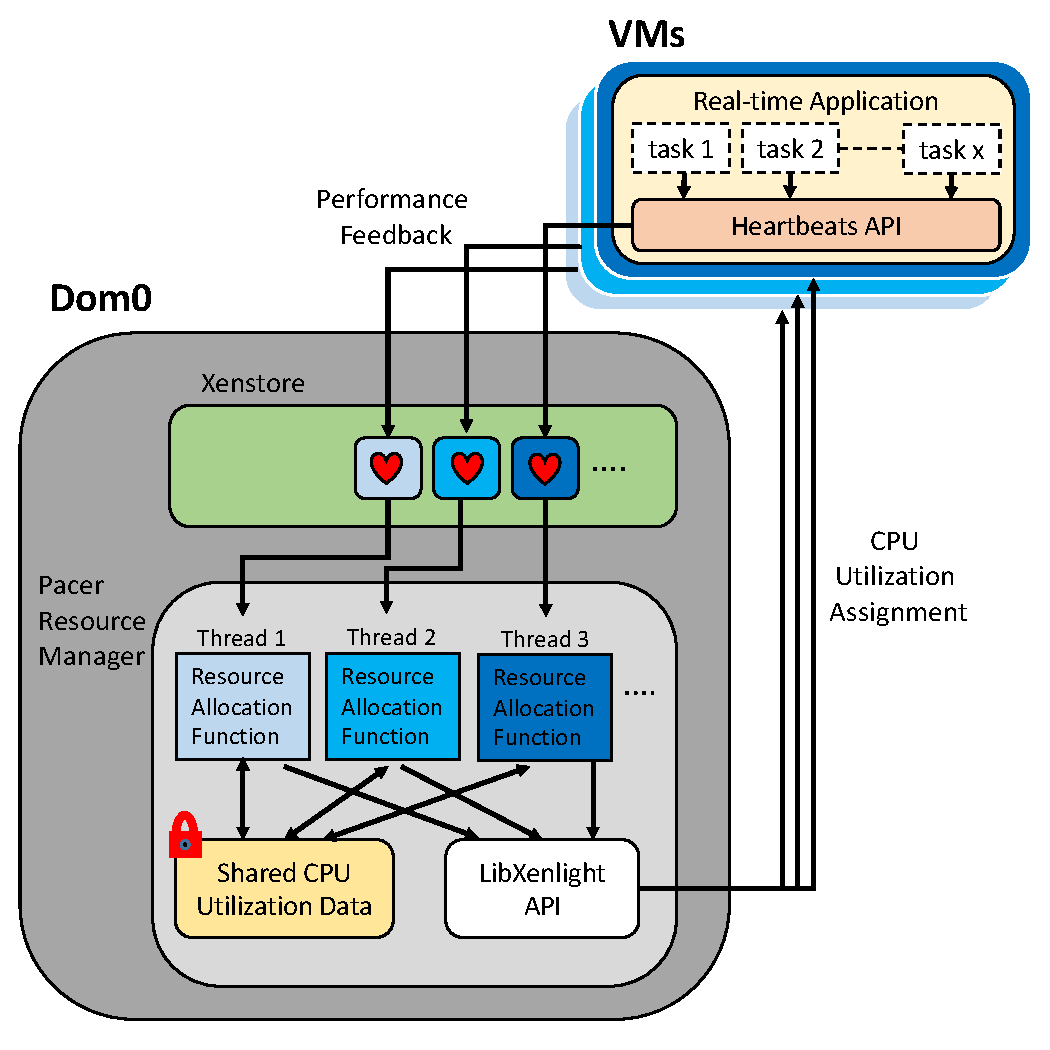
\includegraphics[width=1\linewidth]{images/anchorsd}
\caption{Pacer Framework}
\label{anchorsd}
\end{figure}
